%%----------------------------------------------------------------------------------------
%	PACKAGES AND THEMES
%----------------------------------------------------------------------------------------
\PassOptionsToPackage{table}{xcolor}
\documentclass[aspectratio=169,xcolor=dvipsnames,svgnames,x11names,fleqn]{beamer}
% \documentclass[aspectratio=169,xcolor=dvipsnames,fleqn]{beamer}

\usetheme{RedVelvet}

\usefonttheme[onlymath]{serif}
\newcommand{\showanswers}{yes}


\usepackage{xspace}
\usepackage{amsmath}
\usepackage{amssymb}
\usepackage{amsfonts}
\usepackage{color}
\usepackage{physics}
% \usepackage{mathbb}
\usepackage{rahul_math}
\usepackage{bigints}

\usepackage{graphicx} % Allows including images
\usepackage{booktabs} % Allows the use of \toprule, \midrule and \bottomrule in tables
\usepackage{tikz,pgfplots}

\usepackage{subfigure}
\usetikzlibrary{arrows}
\usepackage{minted}
\definecolor{LightGray}{gray}{0.9}
\definecolor{cream}{rgb}{0.92, 0.9, 0.55}
\definecolor{lightblue}{rgb}{0.68, 0.85, 0.9}


\usepackage{xcolor-material}
\usetikzlibrary{fit}
\usetikzlibrary{matrix}
\tikzset{%
apple/.pic={
    \fill [MaterialBrown] (-1/8,0)  arc (180:120:1 and 3/2) coordinate [pos=3/5] (@)-- ++(1/6,-1/7)  arc (120:180:5/4 and 3/2) -- cycle;
    \fill [MaterialLightGreen500] (0,-9/10)  .. controls ++(180:1/8) and ++(  0:1/4) .. (-1/3,  -1) .. controls ++(180:1/3) and ++(270:1/2) .. (  -1,   0) .. controls ++( 90:1/3) and ++(180:1/3) .. (-1/2, 3/4) .. controls ++(  0:1/8) and ++(135:1/8) .. (   0, 4/7)
    }
    }

\newcommand{\leftdoublequote}{\textcolor{blue}{\scalebox{3}{``}}}

\newcommand{\rightdoublequote}{\textcolor{blue}{\scalebox{3}{''}}}


\usepackage{textcomp}
\usepackage{fontawesome}
\usepackage{tikz,pgfplots}
\usetikzlibrary{shapes.callouts}
\usetikzlibrary{arrows}
\usetikzlibrary{shapes.geometric, positioning}
\pgfplotsset{compat=1.8} % or newest version

\usetikzlibrary{positioning}


\usepackage{bm}
\usepackage{relsize}



\tikzset{basic/.style={draw,fill=MediumBlue!20,text width=1em,text badly centered}}
\tikzset{input/.style={basic,circle}}
\tikzset{weights/.style={basic,rectangle}}
\tikzset{functions/.style={basic,circle,fill=MediumBlue!10}}



\usepackage{listofitems} % for \readlist to create arrays
\tikzstyle{mynode}=[thick,draw=MediumBlue,fill=MediumBlue!20,circle,minimum size=22]


\usepackage{overpic}

%----------------------------------------------------------------------------------------
%	TITLE PAGE
%----------------------------------------------------------------------------------------

\usepackage{tikz-qtree,tikz-qtree-compat}
\usetikzlibrary{tikzmark}
\usetikzlibrary{calc}

\usetikzlibrary{fit}
\tikzset{%
apple/.pic={
    \fill [MaterialBrown] (-1/8,0)  arc (180:120:1 and 3/2) coordinate [pos=3/5] (@)-- ++(1/6,-1/7)  arc (120:180:5/4 and 3/2) -- cycle;
    \fill [MaterialLightGreen500] (0,-9/10)  .. controls ++(180:1/8) and ++(  0:1/4) .. (-1/3,  -1) .. controls ++(180:1/3) and ++(270:1/2) .. (  -1,   0) .. controls ++( 90:1/3) and ++(180:1/3) .. (-1/2, 3/4) .. controls ++(  0:1/8) and ++(135:1/8) .. (   0, 4/7)
}
}
\usepackage{tikz-qtree,tikz-qtree-compat}
\usetikzlibrary{tikzmark}
\usetikzlibrary{calc}

\usetikzlibrary{positioning}


\usepackage{bm}
\usepackage{relsize}



\tikzset{basic/.style={draw,fill=MediumBlue!20,text width=1em,text badly centered}}
\tikzset{input/.style={basic,circle}}
\tikzset{weights/.style={basic,rectangle}}
\tikzset{functions/.style={basic,circle,fill=MediumBlue!10}}



\usepackage{listofitems} % for \readlist to create arrays
\tikzstyle{mynode}=[thick,draw=MediumBlue,fill=MediumBlue!20,circle,minimum size=22]


\newmdenv[
backgroundcolor=androidYellowLight,
linecolor=androidYellow,
linewidth=0.5pt,
roundcorner=10pt,
skipabove=\baselineskip,
skipbelow=\baselineskip
]{MintedFrame}

% Set minted options
\setminted{
fontsize=\footnotesize,
breaklines=true,
autogobble,
linenos,
frame=none
}


\title[CPE 487/587: Deep Learning]{CPE 486/586: Deep Learning for Engineering Applications} % The short title appears at the bottom of every slide, the full title is only on the title page
\subtitle{04 Training Neural Networks  and Computational Thinking}

\author[Rahul Bhadani] {{\Large \textbf{Rahul Bhadani}}}

\institute[UAH] % Your institution as it will appear on the bottom of every slide, maybe shorthand to save space
{
    Electrical \& Computer Engineering,  The University of Alabama in Huntsville
}
\date

% \titlegraphic{
%    \includegraphics[width=0.4\linewidth]{figures/UAH_primary.png}
% }

\begin{document}

%-------------------------------------------------
\begin{frame}
    \titlepage
\end{frame}

%-------------------------------------------------
\begin{frame}{Outline}
    \backgroundtableofcontents
\end{frame}


\section{Recap}

\begin{frame}
    \sectionpage
\end{frame}


\begin{frame}{Linear Layer}

\begin{columns}
\column{0.45\linewidth}


\begin{tikzpicture}[
    % Define styles for the nodes
    input_node/.style={circle, draw=black, fill=blue!30, thick, minimum size=1cm},
    output_node/.style={circle, draw=black, fill=orange!40, thick, minimum size=1cm},
    arrow/.style={-Stealth, thick}
]

    % Input Nodes (x1, x2)
    \node[input_node] (x1) at (0, 3) {$x_1$};
    \node[input_node] (x2) at (0, 1) {$x_2$};
    
    % Ellipsis (Vertical dots)
    \node at (0, -0.2) {\Huge $\vdots$};
    
    % Input Node (xN)
    \node[input_node] (xd) at (0, -1.5) {$x_d$};
    
    % Output Node (y)
    \node[output_node] (y) at (4, 0.75) {$y$};

    % Connections and Labels
    \draw[arrow] (x1) -- (y) node[midway, above right] {$w_1$};
    \draw[arrow] (x2) -- (y) node[midway, above] {$w_2$};
    \draw[arrow] (xd) -- (y) node[midway, below left] {$w_d$};

\end{tikzpicture}


\column{0.45\linewidth}

\pause 

\begin{align*}
y = \sum_{i = 1}^n w_i x_i
\end{align*}


\pause 

\begin{align*}
\wbf = \begin{bmatrix}
w_1 \\ w_2 \\ \vdots \\ w_d
\end{bmatrix} \quad \xbf = \begin{bmatrix}
x_1 & x_2 & \cdots & x_d
\end{bmatrix} 
\end{align*}

\pause 

\begin{align*}
\Rightarrow y = \xbf \wbf
\end{align*}
\end{columns}



\end{frame}



\begin{frame}{Linear Layer: Case of Hidden Layer}

\footnotesize 

\begin{columns}

\column{0.40\linewidth}
\begin{tikzpicture}[
    % Define styles for the nodes
    input_node/.style={circle, draw=black, fill=blue!30, thick, minimum size=1.1cm, inner sep=0pt},
    output_node/.style={circle, draw=black, fill=orange!40, thick, minimum size=1.1cm, inner sep=0pt},
    arrow/.style={-Stealth, thick}
]

    % Input Layer Nodes (x1, x2, ... xn)
    \node[input_node] (x1) at (0, 4) {$x_1$};
    \node[input_node] (x2) at (0, 2) {$x_2$};
    \node at (0, 0.5) {\Huge $\vdots$};
    \node[input_node] (xd) at (0, -1) {$x_d$};
    
    % Output Layer Nodes (z1, ... zM)
    \node[output_node] (z1) at (4, 3) {$z_1$};
    \node at (4, 1.5) {\Huge $\vdots$};
    \node[output_node] (zm) at (4, 0) {$z_m$};

    % Connections from x1
    \draw[arrow] (x1) -- (z1) node[midway, above, sloped] {$w_{11}$};
    \draw[arrow] (x1) -- (zm) node[pos=0.45, right] {$w_{1m}$};

    % Connections from x2
    \draw[arrow] (x2) -- (z1) node[pos=0.2, above] {$w_{21}$};
    \draw[arrow] (x2) -- (zm) node[pos=0.4, left] {$w_{2m}$};

    % Connections from xN
    \draw[arrow] (xd) -- (z1) node[pos=0.3, left] {$w_{d1}$};
    \draw[arrow] (xd) -- (zm) node[midway, below, sloped] {$w_{dm}$};

\end{tikzpicture}

\column{0.55\linewidth}

\pause 
\begin{align*}
z_m = \sum_{i = 1}^n x_i w_{im}
\end{align*}

\pause 

\begin{align*}
\zbf = \begin{bmatrix}
z_1 & z_2 & \vdots & z_m
\end{bmatrix}_{1 \times m} 
\end{align*}

\begin{align*}  W  = \begin{bmatrix}
w_{11} & w_{12} & \cdots & w_{1m}\\
w_{21} & w_{22} & \cdots & w_{2m}\\
\vdots & \vdots & \vdots & \vdots \\
w_{d1} & w_{m2} & \cdots & w_{dm}
\end{bmatrix}_{d \times m} \quad  \xbf = \begin{bmatrix}
x_1 & x_2 & \cdots & x_d
\end{bmatrix}_{1\times d}
\end{align*}

\pause

\begin{align*}
\Rightarrow \zbf = \xbf W
\end{align*}

\end{columns}

\end{frame}


\begin{frame}{Linear Layer: Case of Hidden Layer}

\footnotesize 

\begin{columns}

\column{0.40\linewidth}
\begin{tikzpicture}[
    % Define styles for the nodes
    input_node/.style={circle, draw=black, fill=blue!30, thick, minimum size=1.1cm, inner sep=0pt},
    output_node/.style={circle, draw=black, fill=orange!40, thick, minimum size=1.1cm, inner sep=0pt},
    arrow/.style={-Stealth, thick}
]

    % Input Layer Nodes (x1, x2, ... xn)
    \node[input_node] (x1) at (0, 4) {$x_1$};
    \node[input_node] (x2) at (0, 2) {$x_2$};
    \node at (0, 0.5) {\Huge $\vdots$};
    \node[input_node] (xd) at (0, -1) {$x_d$};
    
    % Output Layer Nodes (z1, ... zM)
    \node[output_node] (z1) at (4, 3) {$z_1$};
    \node at (4, 1.5) {\Huge $\vdots$};
    \node[output_node] (zm) at (4, 0) {$z_m$};

    % Connections from x1
    \draw[arrow] (x1) -- (z1) node[midway, above, sloped] {$w_{11}$};
    \draw[arrow] (x1) -- (zm) node[pos=0.45, right] {$w_{1m}$};

    % Connections from x2
    \draw[arrow] (x2) -- (z1) node[pos=0.2, above] {$w_{21}$};
    \draw[arrow] (x2) -- (zm) node[pos=0.4, left] {$w_{2m}$};

    % Connections from xN
    \draw[arrow] (xd) -- (z1) node[pos=0.3, left] {$w_{d1}$};
    \draw[arrow] (xd) -- (zm) node[midway, below, sloped] {$w_{dm}$};

\end{tikzpicture}

\column{0.55\linewidth}

That was the case of one sample, if we consider $n$ sample, then?


\pause

\begin{align*}
X = \begin{bmatrix}
x_{11} & x_{12} & \cdots & x_{1d}\\
x_{21} & x_{22} & \cdots & x_{2d}\\
\vdots & \vdots & \vdots & \vdots\\
x_{n1} & x_{n2} & \cdots & x_{nd}\\
\end{bmatrix}
\end{align*}

\pause

\begin{align*}
\Rightarrow Z = XW
\end{align*}

\end{columns}

\end{frame}

\begin{frame}{Nonlinear Operation}

\Large

\center

\begin{align*}
A = \sigma(Z)
\end{align*}

which will use elementwise operation.

\end{frame}



\section{Training a Neural Network}

\begin{frame}
    \sectionpage
\end{frame}

\begin{frame}{How to Train your Neural Network}

\begin{center}

\includegraphics[width=0.4\linewidth]{figures/how_to_train_your_nn.jpg}

\tiny 
Image generation from Google Gemini.
\end{center}

\end{frame}


\begin{frame}{Training a Neural Network}

Some criteria to consider:

\footnotesize


\begin{columns}
    \column{0.5\linewidth}

    \begin{enumerate}
\item Data Preprocessing: Normalization/Standardization
%\item Feature Engineering
\item Batch Size
\item Batch Normalization
\item Dropout
\item Early-Stopping
\item Learning-Rate Scheduling
\item Optimizer Selection
    \end{enumerate}

    \column{0.5\linewidth}
\begin{enumerate}
    \setcounter{enumi}{7}
    \item Weight Initialization
\item Activation Functions
\item Network Depth \& Width
\item Skip/Residual Connections
\item Regularization
\item Loss Functions
\item Gradient Clipping
\item Warm-Up Scheduling
\end{enumerate}

\end{columns}



\end{frame}

\subsection{Data Preprocessing}

\begin{frame}
    \subsectionpage
\end{frame}

\begin{frame}{Imputing Missing Values}


\begin{facts}{Definition}

The process of filling miss values or correct known errors is called \textbf{imputation}.

\end{facts}

\tiny

\begin{figure}[h]
\centering
\begin{tikzpicture}[scale=0.9]
    % Define colors
    \definecolor{headerBg}{RGB}{200, 220, 255}
    \definecolor{nanColor}{RGB}{255, 200, 200}
    \definecolor{dataColor}{RGB}{240, 248, 255}
    
    % Table parameters
    \def\cellw{1.2}
    \def\cellh{0.6}
    \def\sx{2}
    \def\sy{0}
    
    % ===== HEADER ROW =====
    \draw[fill=headerBg, draw=black, line width=1pt] 
        (\sx + 1*\cellw, \sy) rectangle (\sx + 2*\cellw, \sy + \cellh);
    \node at (\sx + 1.5*\cellw, \sy + \cellh/2) {\small $x_1$};
    
    \draw[fill=headerBg, draw=black, line width=1pt] 
        (\sx + 2*\cellw, \sy) rectangle (\sx + 3*\cellw, \sy + \cellh);
    \node at (\sx + 2.5*\cellw, \sy + \cellh/2) {\small $x_2$};
    
    \draw[fill=headerBg, draw=black, line width=1pt] 
        (\sx + 3*\cellw, \sy) rectangle (\sx + 4*\cellw, \sy + \cellh);
    \node at (\sx + 3.5*\cellw, \sy + \cellh/2) {\small $x_3$};
    
    \draw[fill=headerBg, draw=black, line width=1pt] 
        (\sx + 4*\cellw, \sy) rectangle (\sx + 5*\cellw, \sy + \cellh);
    \node at (\sx + 4.5*\cellw, \sy + \cellh/2) {\small $x_4$};
    
    \draw[fill=headerBg, draw=black, line width=1pt] 
        (\sx + 5*\cellw, \sy) rectangle (\sx + 6*\cellw, \sy + \cellh);
    \node at (\sx + 5.5*\cellw, \sy + \cellh/2) {\small $x_5$};
    
    % ===== ROW 0: Sample 0 =====
    \node[anchor=east, font=\small\bfseries] at (\sx - 0.3, \sy - 1*\cellh + \cellh/2) {Sample 0};
    
    \draw[fill=dataColor, draw=black, line width=0.5pt] (\sx + 1*\cellw, \sy - 1*\cellh) rectangle (\sx + 2*\cellw, \sy - 1*\cellh + \cellh);
    \node at (\sx + 1.5*\cellw, \sy - 1*\cellh + \cellh/2) {\footnotesize 2.3};
    
    \draw[fill=dataColor, draw=black, line width=0.5pt] (\sx + 2*\cellw, \sy - 1*\cellh) rectangle (\sx + 3*\cellw, \sy - 1*\cellh + \cellh);
    \node at (\sx + 2.5*\cellw, \sy - 1*\cellh + \cellh/2) {\footnotesize 4.1};
    
    \draw[fill=nanColor, draw=black, line width=0.5pt] (\sx + 3*\cellw, \sy - 1*\cellh) rectangle (\sx + 4*\cellw, \sy - 1*\cellh + \cellh);
    \node at (\sx + 3.5*\cellw, \sy - 1*\cellh + \cellh/2) {\footnotesize NaN};
    
    \draw[fill=dataColor, draw=black, line width=0.5pt] (\sx + 4*\cellw, \sy - 1*\cellh) rectangle (\sx + 5*\cellw, \sy - 1*\cellh + \cellh);
    \node at (\sx + 4.5*\cellw, \sy - 1*\cellh + \cellh/2) {\footnotesize 3.7};
    
    \draw[fill=dataColor, draw=black, line width=0.5pt] (\sx + 5*\cellw, \sy - 1*\cellh) rectangle (\sx + 6*\cellw, \sy - 1*\cellh + \cellh);
    \node at (\sx + 5.5*\cellw, \sy - 1*\cellh + \cellh/2) {\footnotesize 1.9};
    
    % ===== ROW 1: Sample 1 =====
    \node[anchor=east, font=\small\bfseries] at (\sx - 0.3, \sy - 2*\cellh + \cellh/2) {Sample 1};
    
    \draw[fill=dataColor, draw=black, line width=0.5pt] (\sx + 1*\cellw, \sy - 2*\cellh) rectangle (\sx + 2*\cellw, \sy - 2*\cellh + \cellh);
    \node at (\sx + 1.5*\cellw, \sy - 2*\cellh + \cellh/2) {\footnotesize 5.2};
    
    \draw[fill=nanColor, draw=black, line width=0.5pt] (\sx + 2*\cellw, \sy - 2*\cellh) rectangle (\sx + 3*\cellw, \sy - 2*\cellh + \cellh);
    \node at (\sx + 2.5*\cellw, \sy - 2*\cellh + \cellh/2) {\footnotesize NaN};
    
    \draw[fill=dataColor, draw=black, line width=0.5pt] (\sx + 3*\cellw, \sy - 2*\cellh) rectangle (\sx + 4*\cellw, \sy - 2*\cellh + \cellh);
    \node at (\sx + 3.5*\cellw, \sy - 2*\cellh + \cellh/2) {\footnotesize 2.8};
    
    \draw[fill=dataColor, draw=black, line width=0.5pt] (\sx + 4*\cellw, \sy - 2*\cellh) rectangle (\sx + 5*\cellw, \sy - 2*\cellh + \cellh);
    \node at (\sx + 4.5*\cellw, \sy - 2*\cellh + \cellh/2) {\footnotesize 1.5};
    
    \draw[fill=dataColor, draw=black, line width=0.5pt] (\sx + 5*\cellw, \sy - 2*\cellh) rectangle (\sx + 6*\cellw, \sy - 2*\cellh + \cellh);
    \node at (\sx + 5.5*\cellw, \sy - 2*\cellh + \cellh/2) {\footnotesize 4.3};
    
    % ===== ROW 2: Sample 2 =====
    \node[anchor=east, font=\small\bfseries] at (\sx - 0.3, \sy - 3*\cellh + \cellh/2) {Sample 2};
    
    \draw[fill=dataColor, draw=black, line width=0.5pt] (\sx + 1*\cellw, \sy - 3*\cellh) rectangle (\sx + 2*\cellw, \sy - 3*\cellh + \cellh);
    \node at (\sx + 1.5*\cellw, \sy - 3*\cellh + \cellh/2) {\footnotesize 1.1};
    
    \draw[fill=dataColor, draw=black, line width=0.5pt] (\sx + 2*\cellw, \sy - 3*\cellh) rectangle (\sx + 3*\cellw, \sy - 3*\cellh + \cellh);
    \node at (\sx + 2.5*\cellw, \sy - 3*\cellh + \cellh/2) {\footnotesize 3.4};
    
    \draw[fill=dataColor, draw=black, line width=0.5pt] (\sx + 3*\cellw, \sy - 3*\cellh) rectangle (\sx + 4*\cellw, \sy - 3*\cellh + \cellh);
    \node at (\sx + 3.5*\cellw, \sy - 3*\cellh + \cellh/2) {\footnotesize 2.6};
    
    \draw[fill=nanColor, draw=black, line width=0.5pt] (\sx + 4*\cellw, \sy - 3*\cellh) rectangle (\sx + 5*\cellw, \sy - 3*\cellh + \cellh);
    \node at (\sx + 4.5*\cellw, \sy - 3*\cellh + \cellh/2) {\footnotesize NaN};
    
    \draw[fill=dataColor, draw=black, line width=0.5pt] (\sx + 5*\cellw, \sy - 3*\cellh) rectangle (\sx + 6*\cellw, \sy - 3*\cellh + \cellh);
    \node at (\sx + 5.5*\cellw, \sy - 3*\cellh + \cellh/2) {\footnotesize 5.1};
    
    % ===== ROW 3: Sample 3 =====
    \node[anchor=east, font=\small\bfseries] at (\sx - 0.3, \sy - 4*\cellh + \cellh/2) {Sample 3};
    
    \draw[fill=nanColor, draw=black, line width=0.5pt] (\sx + 1*\cellw, \sy - 4*\cellh) rectangle (\sx + 2*\cellw, \sy - 4*\cellh + \cellh);
    \node at (\sx + 1.5*\cellw, \sy - 4*\cellh + \cellh/2) {\footnotesize NaN};
    
    \draw[fill=dataColor, draw=black, line width=0.5pt] (\sx + 2*\cellw, \sy - 4*\cellh) rectangle (\sx + 3*\cellw, \sy - 4*\cellh + \cellh);
    \node at (\sx + 2.5*\cellw, \sy - 4*\cellh + \cellh/2) {\footnotesize 2.2};
    
    \draw[fill=dataColor, draw=black, line width=0.5pt] (\sx + 3*\cellw, \sy - 4*\cellh) rectangle (\sx + 4*\cellw, \sy - 4*\cellh + \cellh);
    \node at (\sx + 3.5*\cellw, \sy - 4*\cellh + \cellh/2) {\footnotesize 4.0};
    
    \draw[fill=dataColor, draw=black, line width=0.5pt] (\sx + 4*\cellw, \sy - 4*\cellh) rectangle (\sx + 5*\cellw, \sy - 4*\cellh + \cellh);
    \node at (\sx + 4.5*\cellw, \sy - 4*\cellh + \cellh/2) {\footnotesize 3.3};
    
    \draw[fill=dataColor, draw=black, line width=0.5pt] (\sx + 5*\cellw, \sy - 4*\cellh) rectangle (\sx + 6*\cellw, \sy - 4*\cellh + \cellh);
    \node at (\sx + 5.5*\cellw, \sy - 4*\cellh + \cellh/2) {\footnotesize 2.9};
    
    % ===== ROW 4: Sample 4 =====
    \node[anchor=east, font=\small\bfseries] at (\sx - 0.3, \sy - 5*\cellh + \cellh/2) {Sample 4};
    
    \draw[fill=dataColor, draw=black, line width=0.5pt] (\sx + 1*\cellw, \sy - 5*\cellh) rectangle (\sx + 2*\cellw, \sy - 5*\cellh + \cellh);
    \node at (\sx + 1.5*\cellw, \sy - 5*\cellh + \cellh/2) {\footnotesize 3.5};
    
    \draw[fill=dataColor, draw=black, line width=0.5pt] (\sx + 2*\cellw, \sy - 5*\cellh) rectangle (\sx + 3*\cellw, \sy - 5*\cellh + \cellh);
    \node at (\sx + 2.5*\cellw, \sy - 5*\cellh + \cellh/2) {\footnotesize 1.8};
    
    \draw[fill=dataColor, draw=black, line width=0.5pt] (\sx + 3*\cellw, \sy - 5*\cellh) rectangle (\sx + 4*\cellw, \sy - 5*\cellh + \cellh);
    \node at (\sx + 3.5*\cellw, \sy - 5*\cellh + \cellh/2) {\footnotesize 2.1};
    
    \draw[fill=dataColor, draw=black, line width=0.5pt] (\sx + 4*\cellw, \sy - 5*\cellh) rectangle (\sx + 5*\cellw, \sy - 5*\cellh + \cellh);
    \node at (\sx + 4.5*\cellw, \sy - 5*\cellh + \cellh/2) {\footnotesize 4.5};
    
    \draw[fill=nanColor, draw=black, line width=0.5pt] (\sx + 5*\cellw, \sy - 5*\cellh) rectangle (\sx + 6*\cellw, \sy - 5*\cellh + \cellh);
    \node at (\sx + 5.5*\cellw, \sy - 5*\cellh + \cellh/2) {\footnotesize NaN};
    
    % ===== ROW 5: Sample 5 =====
    \node[anchor=east, font=\small\bfseries] at (\sx - 0.3, \sy - 6*\cellh + \cellh/2) {Sample 5};
    
    \draw[fill=dataColor, draw=black, line width=0.5pt] (\sx + 1*\cellw, \sy - 6*\cellh) rectangle (\sx + 2*\cellw, \sy - 6*\cellh + \cellh);
    \node at (\sx + 1.5*\cellw, \sy - 6*\cellh + \cellh/2) {\footnotesize 2.7};
    
    \draw[fill=dataColor, draw=black, line width=0.5pt] (\sx + 2*\cellw, \sy - 6*\cellh) rectangle (\sx + 3*\cellw, \sy - 6*\cellh + \cellh);
    \node at (\sx + 2.5*\cellw, \sy - 6*\cellh + \cellh/2) {\footnotesize 3.9};
    
    \draw[fill=nanColor, draw=black, line width=0.5pt] (\sx + 3*\cellw, \sy - 6*\cellh) rectangle (\sx + 4*\cellw, \sy - 6*\cellh + \cellh);
    \node at (\sx + 3.5*\cellw, \sy - 6*\cellh + \cellh/2) {\footnotesize NULL};
    
    \draw[fill=dataColor, draw=black, line width=0.5pt] (\sx + 4*\cellw, \sy - 6*\cellh) rectangle (\sx + 5*\cellw, \sy - 6*\cellh + \cellh);
    \node at (\sx + 4.5*\cellw, \sy - 6*\cellh + \cellh/2) {\footnotesize 1.2};
    
    \draw[fill=dataColor, draw=black, line width=0.5pt] (\sx + 5*\cellw, \sy - 6*\cellh) rectangle (\sx + 6*\cellw, \sy - 6*\cellh + \cellh);
    \node at (\sx + 5.5*\cellw, \sy - 6*\cellh + \cellh/2) {\footnotesize 4.6};
    
    % ===== FEATURE INDEX ARROW (above) =====
    \draw[-{Latex[length=3mm, width=2mm]}, line width=2pt, color=blue] 
        (\sx + 1.5*\cellw, \sy + 1.5*\cellh) -- (\sx + 5.5*\cellw, \sy + 1.5*\cellh);
    \node[anchor=south, font=\large, color=blue] 
        at (\sx + 3.5*\cellw, \sy + 1.8*\cellh) {Feature Index};
    
    % ===== SAMPLE INDEX ARROW (left side, rotated) =====
    \draw[-{Latex[length=3mm, width=2mm]}, line width=2pt, color=red] 
        (\sx + 0.8, \sy - 0.5*\cellh) -- (\sx + 0.8, \sy - 5.5*\cellh);
    \node[rotate=90, anchor=south, font=\large, color=red] 
        at (\sx + 0.5, \sy - 3*\cellh) {Sample Index};
    
    % ===== LEGEND BOX =====
    \begin{scope}[xshift=12cm, yshift=-1cm]
        \draw[fill=white, draw=black, line width=1.5pt, rounded corners=3pt] 
            (0, 0) rectangle (4, 2.5);
        
        \node[anchor=west, font=\bfseries] at (0.2, 2) {Legend:};
        
        \draw[fill=headerBg, draw=black] (0.2, 1.5) rectangle (0.6, 1.8);
        \node[anchor=west, font=\small] at (0.8, 1.65) {Feature header};
        
        \draw[fill=dataColor, draw=black] (0.2, 1.0) rectangle (0.6, 1.3);
        \node[anchor=west, font=\small] at (0.8, 1.15) {Valid data};
        
        \draw[fill=nanColor, draw=black] (0.2, 0.5) rectangle (0.6, 0.8);
        \node[anchor=west, font=\small] at (0.8, 0.65) {Missing (NaN)};
    \end{scope}
    
    
    
\end{tikzpicture}
\caption{Data Table Structure: Features as Columns, Samples as Rows. 
Red cells indicate missing values (NaN) that require imputation before model training.}
\end{figure}


\end{frame}


\begin{frame}{Common Types of Missing Values}

\begin{enumerate}

\item Missing Completely at Random (MCAR), i.e. the probability
of being missing is not related to the data and is only dependent on some parameter $\phi$.

\item Missing at Random (MAR), i.e., the missingness probability is only related to the observed variables in the data.

\item Missing not at random (MNAR), neither of the above, and  the missingness probability is related to missing values of the
incomplete variable, which are unknown to us, even after conditioning on observed information

\end{enumerate}

\end{frame}


\begin{frame}{Common Imputation Methods}

\begin{enumerate}

\item Get rid of those samples where missing \# features exceed certain number (or percentage)
\item Get rid of feaures where \# missing values exceed certai numbers (or percentage)
\item Sample Mean (only for continuous data)
\item Sample Median (only for continuous data) 
\item k-Nearest Neighbors (kNN) imputation
\item Expectation-Maximization (EM) imputation
\item Bayesian Approach
\end{enumerate}

\begin{tblock}{}
Mean and median approach or anything similar would fail to quantify uncertainty in the estimated missing value.
\end{tblock}

\end{frame}

\begin{frame}{Bayesian Estimation for Missing Data}

\begin{gradbox}{}

\begin{enumerate}

\item Model your data first (probabilistic modeling): e.g. normal distribution.

\item Compute prior distribution over uknown parameters.
\item Calculate posterior: update the prior using observed data as (Bayes' Theorem in the play). This gives a posterior distribution over model parameters and missing values.
\item Draw samples using Markov Chain Monte Carlo simulation that will be plausible missing values.

\begin{center}
{\bf\color{SeaGreen4}Under a Bayesian framework, missing observations can be thought of as any other parameter in the model whose distribution needs to be determined.}
\end{center}

\end{enumerate}
\end{gradbox} 
 
\end{frame}

\begin{frame}{Bayesian Framework}

\small

\begin{tcolorbox}[title=Posterior Distribution, colframe=pink]

\begin{align*}
p(\boldsymbol{\theta} \mid X) = \frac{p(\mathbf{X} \mid \boldsymbol{\theta}) \, p(\boldsymbol{\theta})}{\int_{-\infty}^{\infty} p(\mathbf{X} \mid \boldsymbol{\theta}) \, p(\boldsymbol{\theta}) \, d\boldsymbol{\theta}}  \propto p(\mathbf{X} \mid \boldsymbol{\theta}) \, p(\boldsymbol{\theta})
\end{align*}

$p(\mathbf{X} \mid \boldsymbol{\theta})$ is likelihood, $p(\boldsymbol{\theta})$ is prior.



\end{tcolorbox}

\begin{align*}
p(\mathbf{X}_{mis} \mid \mathbf{X}_{obs}) = \int p(\mathbf{X}_{mis} \mid \mathbf{X}_{obs}, \boldsymbol{\theta}) \, p(\boldsymbol{\theta} \mid \mathbf{X}_{obs}) \, d\boldsymbol{\theta}.
\end{align*}

Calculating posterior is hard, so we use Monte Carlo methods (Markov Chain Monte Carlo (MCMC)).

\footnotesize 

An example code for MCMC imputation using PyMC is available at {\url{https://www.pymc.io/projects/examples/en/latest/howto/Missing_Data_Imputation.html}}
\end{frame}


\begin{frame}{Normalization/Standardization}

\begin{tcolorbox}[title=Definition, colframe=pink, colback=NavajoWhite1]
In simpler terms: adjusting values measured on different scales to a common scale is \textbf{Normalization}.

\bigskip

Otherwise, aligning entire probability distribution of adjusted values is \textbf{Normalization}.


\end{tcolorbox}


\begin{columns}
    \column{0.5\linewidth}

    \begin{tcolorbox}[colframe=lightblue, title=Standard Normalization]
        \begin{align*}
            \xhat = \frac{x - \mu}{\sigma}
        \end{align*}
    \end{tcolorbox}

    \column{0.5\linewidth}

    \begin{tcolorbox}[colframe=Green!60, title=Minmax Normalization]
        \begin{align*}
            \xhat = \frac{x - x_{min}}{ x_{max} -  x_{min}}
        \end{align*}
    \end{tcolorbox}
    
\end{columns}


\end{frame}


\subsection{Impact of Batch Size in the Training Process}

\begin{frame}
    \subsectionpage
\end{frame}


\begin{frame}{Batch Size}

    \begin{tcolorbox}[title=Definition, colframe=Orange!30, colback=Green!10]
    The number of samples passed through the neural network simultaneously is called \textbf{batch size}.
    \end{tcolorbox}
    
    Determining a suitable batch size is an important consideration to the training process, as it may influence the learning rate of the model. 
    
    \begin{center}
    \begin{align*}
    \wbf = \wbf - \eta \frac{1}{m}\sum_{i=1}^m \nabla_\wbf \Lcal_i(\wbf)
    \end{align*}
    \end{center}
    

    $m$ is the batch size.

\end{frame}

\begin{frame}{}
    
    \begin{center}
        \begin{forest}{}
            \LARGE \centering
        How does the batch size affect training?
        \end{forest}

    \end{center}
    
\end{frame}

\begin{frame}{Stochastic Gradient Descent and Batch Size}
    
    \Large 
    {\faQuestionCircle~~ What's problem if we use entire training set for gradient descent? }

    \pause 

    \vspace{10pt}

    \begin{tblock}{}
        Stochastic gradient descent provides approximation of true gradients using one sample at a time after shuffling the training sample and pick one training sample to update the weights. It optionally adds a small noise to the gradient calculation.
    \end{tblock}
    

\end{frame}

\begin{frame}{Mini Batch}
    
    Single sample gradient calculation can be very slow, so we can choose more than one sample at a time (but not all of them). This is called \textbf{mini batch}.

\end{frame}

\begin{frame}{Suggested Reading}

    \large 
    \begin{enumerate}
        \item Masters, Dominic, and Carlo Luschi. \textbf{"Revisiting small batch training for deep neural networks."} arXiv preprint arXiv:1804.07612 (2018).
        \item You, Yang, Yuhui Wang, Huan Zhang, Zhao Zhang, James Demmel, and Cho-Jui Hsieh. \textbf{"The limit of the batch size."} arXiv preprint arXiv:2006.08517 (2020).
        \item Smith, Samuel L., Pieter-Jan Kindermans, Chris Ying, and Quoc V. Le. \textbf{"Don't decay the learning rate, increase the batch size."} arXiv preprint arXiv:1711.00489 (2017).
    \end{enumerate}
    
\end{frame}

\begin{frame}{Batch Normalization}

    Normalization applied per batch:

    \begin{align*}
        \hat{\xbf}_i = \frac{\xbf_i - \mu_{\Bcal}}{\sqrt{\sigma^2_\Bcal + \epsilon}}
    \end{align*}
    
    $ \mu_{\Bcal}$ batchwise mean, $\sigma^2_\Bcal$ is batchwise variance, and $\epsilon$ is to avoid numerical instability.
\end{frame}

\begin{frame}{Batch Normalization}
    But why Batch Normalization?

    \pause 

    \begin{enumerate}
        \item Batch Normalization smoothened out the loss landscape.
        \item Gradients become more reliable and predictive.
    \end{enumerate}

    \bigskip

    \small

\textbf{Reading:}

    \footnotesize


\begin{enumerate}
    \item Santurkar, Shibani, Dimitris Tsipras, Andrew Ilyas, and Aleksander Madry. \textbf{"How does batch normalization help optimization?."} Advances in neural information processing systems 31 (2018).
    \item Section 3.3 of Huang, Lei. Normalization Techniques in Deep Learning. Cham: Springer, 2022.
\end{enumerate}

\end{frame}


\subsection{Preventing Overfitting and Regularization}

\begin{frame}
    \subsectionpage
\end{frame}


%------------------------------------------------
\begin{frame}{Dropout}

\begin{tblock}{Dropout: A new way to regularize a network}
\begin{itemize}
    \item The central idea behind {\em\color{MediumBlue}dropout} is to randomly dropout nodes in the neural network with a probability $p$. After the nodes are ``dropped out'' the remain network is a subnetwork of the original. 
    \item Dropout has been shown to work quite well at preventing overfitting and allowing the network to find a good local minimum. 
    \item {\bf\color{MediumRed}Recommendation}: Use dropout! 
\end{itemize}
\end{tblock}
{\footnotesize
Nitish Srivastava, Geoffrey Hinton, Alex Krizhevsky, Ilya Sutskever, Ruslan Salakhutdinov, ``Dropout: A Simple Way to Prevent Neural Networks from Overfitting,'' {\em Journal of Machine Learning Research}, 15(56):1929--1958, 2014.}
\end{frame}


%------------------------------------------------
\begin{frame}{Dropout in a Neural Network}

\begin{center}
    
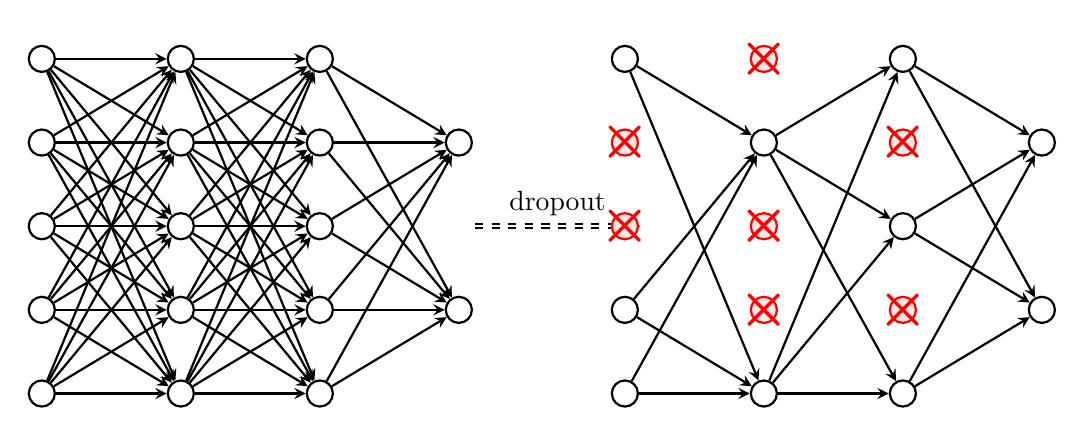
\begin{tikzpicture}

	\node[circle, draw, thick] (i1) {};
	\node[circle, draw, thick, above=2em of i1] (i2) {};
	\node[circle, draw, thick, above=2em of i2] (i3) {};
	\node[circle, draw, thick, below=2em of i1] (i4) {};
	\node[circle, draw, thick, below=2em of i4] (i5) {};
	
	\node[circle, draw, thick, right=4em of i1] (h1) {};
	\node[circle, draw, thick, right=4em of i2] (h2) {};
	\node[circle, draw, thick, right=4em of i3] (h3) {};
	\node[circle, draw, thick, right=4em of i4] (h4) {};
	\node[circle, draw, thick, right=4em of i5] (h5) {};
	
	\node[circle, draw, thick, right=4em of h1] (hh1) {};
	\node[circle, draw, thick, right=4em of h2] (hh2) {};
	\node[circle, draw, thick, right=4em of h3] (hh3) {};
	\node[circle, draw, thick, right=4em of h4] (hh4) {};
	\node[circle, draw, thick, right=4em of h5] (hh5) {};
	
	\node[circle, draw, thick, right=4em of hh2] (o1) {};
	\node[circle, draw, thick, right=4em of hh4] (o2) {};
	
	\draw[-stealth, thick] (i1) -- (h1);
	\draw[-stealth, thick] (i1) -- (h2);
	\draw[-stealth, thick] (i1) -- (h3);
	\draw[-stealth, thick] (i1) -- (h4);
	\draw[-stealth, thick] (i1) -- (h5);
	\draw[-stealth, thick] (i2) -- (h1);
	\draw[-stealth, thick] (i2) -- (h2);
	\draw[-stealth, thick] (i2) -- (h3);
	\draw[-stealth, thick] (i2) -- (h4);
	\draw[-stealth, thick] (i2) -- (h5);
	\draw[-stealth, thick] (i3) -- (h1);
	\draw[-stealth, thick] (i3) -- (h2);
	\draw[-stealth, thick] (i3) -- (h3);
	\draw[-stealth, thick] (i3) -- (h4);
	\draw[-stealth, thick] (i3) -- (h5);
	\draw[-stealth, thick] (i4) -- (h1);
	\draw[-stealth, thick] (i4) -- (h2);
	\draw[-stealth, thick] (i4) -- (h3);
	\draw[-stealth, thick] (i4) -- (h4);
	\draw[-stealth, thick] (i4) -- (h5);
	\draw[-stealth, thick] (i5) -- (h1);
	\draw[-stealth, thick] (i5) -- (h2);
	\draw[-stealth, thick] (i5) -- (h3);
	\draw[-stealth, thick] (i5) -- (h4);
	\draw[-stealth, thick] (i5) -- (h5);
	
	\draw[-stealth, thick] (h1) -- (hh1);
	\draw[-stealth, thick] (h1) -- (hh2);
	\draw[-stealth, thick] (h1) -- (hh3);
	\draw[-stealth, thick] (h1) -- (hh4);
	\draw[-stealth, thick] (h1) -- (hh5);
	\draw[-stealth, thick] (h2) -- (hh1);
	\draw[-stealth, thick] (h2) -- (hh2);
	\draw[-stealth, thick] (h2) -- (hh3);
	\draw[-stealth, thick] (h2) -- (hh4);
	\draw[-stealth, thick] (h2) -- (hh5);
	\draw[-stealth, thick] (h3) -- (hh1);
	\draw[-stealth, thick] (h3) -- (hh2);
	\draw[-stealth, thick] (h3) -- (hh3);
	\draw[-stealth, thick] (h3) -- (hh4);
	\draw[-stealth, thick] (h3) -- (hh5);
	\draw[-stealth, thick] (h4) -- (hh1);
	\draw[-stealth, thick] (h4) -- (hh2);
	\draw[-stealth, thick] (h4) -- (hh3);
	\draw[-stealth, thick] (h4) -- (hh4);
	\draw[-stealth, thick] (h4) -- (hh5);
	\draw[-stealth, thick] (h5) -- (hh1);
	\draw[-stealth, thick] (h5) -- (hh2);
	\draw[-stealth, thick] (h5) -- (hh3);
	\draw[-stealth, thick] (h5) -- (hh4);
	\draw[-stealth, thick] (h5) -- (hh5);
	
	
	\draw[-stealth, thick] (hh1) -- (o1);
	\draw[-stealth, thick] (hh1) -- (o2);
	\draw[-stealth, thick] (hh2) -- (o1);
	\draw[-stealth, thick] (hh2) -- (o2);
	\draw[-stealth, thick] (hh3) -- (o1);
	\draw[-stealth, thick] (hh3) -- (o2);
	\draw[-stealth, thick] (hh4) -- (o1);
	\draw[-stealth, thick] (hh4) -- (o2);
	\draw[-stealth, thick] (hh5) -- (o1);
	\draw[-stealth, thick] (hh5) -- (o2);
	
	\draw[-stealth, double, dashed, thick] (5.5,0) -- node[above] {dropout} (7.6, 0);
	
	
	%%% BOUNDARY %%%
	
	\node[circle, draw, thick, red, fill=red!10, right=10em of hh1] (i1) {};
	\node[circle, draw, thick, red, fill=red!10, above=2em of i1] (i2) {};
	\node[circle, draw, thick, above=2em of i2] (i3) {};
	\node[circle, draw, thick, below=2em of i1] (i4) {};
	\node[circle, draw, thick, below=2em of i4] (i5) {};
	
	\node[red] (icr) at (i1) {$\mathlarger{\mathlarger{\mathlarger{\mathlarger{\mathlarger{\bm{\times}}}}}}$};
	\node[red] (icr) at (i2) {$\mathlarger{\mathlarger{\mathlarger{\mathlarger{\mathlarger{\bm{\times}}}}}}$};
	
	\node[circle, draw, thick, red, fill=red!10, right=4em of i1] (h1) {};
	\node[circle, draw, thick, right=4em of i2] (h2) {};
	\node[circle, draw, thick, red, fill=red!10, right=4em of i3] (h3) {};
	\node[circle, draw, thick, red, fill=red!10, right=4em of i4] (h4) {};
	\node[circle, draw, thick, right=4em of i5] (h5) {};
	
	\node[red] (icr) at (h1) {$\mathlarger{\mathlarger{\mathlarger{\mathlarger{\mathlarger{\bm{\times}}}}}}$};
	\node[red] (icr) at (h3) {$\mathlarger{\mathlarger{\mathlarger{\mathlarger{\mathlarger{\bm{\times}}}}}}$};
	\node[red] (icr) at (h4) {$\mathlarger{\mathlarger{\mathlarger{\mathlarger{\mathlarger{\bm{\times}}}}}}$};
	
	\node[circle, draw, thick, right=4em of h1] (hh1) {};
	\node[circle, draw, thick, red, fill=red!10, right=4em of h2] (hh2) {};
	\node[circle, draw, thick, right=4em of h3] (hh3) {};
	\node[circle, draw, thick, red, fill=red!10, right=4em of h4] (hh4) {};
	\node[circle, draw, thick, right=4em of h5] (hh5) {};
	
	\node[red] (icr) at (hh2) {$\mathlarger{\mathlarger{\mathlarger{\mathlarger{\mathlarger{\bm{\times}}}}}}$};
	\node[red] (icr) at (hh4) {$\mathlarger{\mathlarger{\mathlarger{\mathlarger{\mathlarger{\bm{\times}}}}}}$};
	
	\node[circle, draw, thick, right=4em of hh2] (o1) {};
	\node[circle, draw, thick, right=4em of hh4] (o2) {};
	
	\draw[-stealth, thick] (i3) -- (h2);
	\draw[-stealth, thick] (i3) -- (h5);
	\draw[-stealth, thick] (i4) -- (h2);
	\draw[-stealth, thick] (i4) -- (h5);
	\draw[-stealth, thick] (i5) -- (h2);
	\draw[-stealth, thick] (i5) -- (h5);
	
	\draw[-stealth, thick] (h2) -- (hh1);
	\draw[-stealth, thick] (h2) -- (hh3);
	\draw[-stealth, thick] (h2) -- (hh5);
	\draw[-stealth, thick] (h5) -- (hh1);
	\draw[-stealth, thick] (h5) -- (hh3);
	\draw[-stealth, thick] (h5) -- (hh5);
	
	\draw[-stealth, thick] (hh1) -- (o1);
	\draw[-stealth, thick] (hh1) -- (o2);
	\draw[-stealth, thick] (hh3) -- (o1);
	\draw[-stealth, thick] (hh3) -- (o2);
	\draw[-stealth, thick] (hh5) -- (o1);
	\draw[-stealth, thick] (hh5) -- (o2);

\end{tikzpicture}



\end{center}

\end{frame}


\begin{frame}{Dropout Model}

    \footnotesize

During training, Dropout stochastically "thins" the network by sampling a mask from a Bernoulli distribution.

    \begin{mybox}{}
        \begin{align*}
        r_i^{(l)} &\sim \text{Bernoulli}(p) \tag{Mask} \\
        \mathbf{\tilde{y}}^{(l)} &= \mathbf{r}^{(l)} \otimes \mathbf{y}^{(l)} \tag{Thinned Output} \\
        \mathbf{z}^{(l+1)} &= W^{(l+1)}\mathbf{\tilde{y}}^{(l)} + \mathbf{b}^{(l+1)} \\
        \mathbf{y}^{(l+1)} &= \sigma(\mathbf{z}^{(l+1)})
        \end{align*}
    \end{mybox}
\footnotesize
    \begin{itemize}
        \item $\mathbf{r}^{(l)}$ is a vector of independent Bernoulli random variables, each of which has probability $p$ of being $1$.
        \item The operator $\otimes$ denotes an element-wise product.
        \item $\sigma$ is an activation function.
        \item The thinned outputs as input to the next layer. 
        \item For learning, the derivatives of the loss function are backpropagated through the thinned network.
        \item At test time, the weights are scaled as $W^{(l)}_{test} = pW^{(l)}$. The resulting neural network is run without
dropout.
    \end{itemize}
\end{frame}


\begin{frame}{Regularization in Neural Network}

    \begin{columns}
        \column{0.45\linewidth}

        \begin{tcolorbox}[colframe=Indigo!20, colback=purple!10, title=L2 Regularization]
            \begin{align*}
                \hat{\Lcal}(W) = \Lcal(W)+ \frac{\alpha}{2} ||W||^2_2
            \end{align*}
        \end{tcolorbox}

        \column{0.45\linewidth}

        \begin{tcolorbox}[colframe=Blue!20, colback=Green!10, title=L1 Regularization]
            \begin{align*}
                \hat{\Lcal}(W) = \Lcal(W)+ \frac{\beta}{2} ||W||_1
            \end{align*}
        \end{tcolorbox}
        
        

    \end{columns}

    \begin{enumerate}
            \item L1 regularization promotes sparsity by forcing weights to zero.
            \item L2 regularization shrinks weights, but some of the components of weights large than others that are contributing more to the model.
        \end{enumerate}
    
\end{frame}


\subsection{Network Architecture Consideration}

\begin{frame}
    \subsectionpage
\end{frame}

\begin{frame}{Skip/Residual Connection}

    A shallower layer directly connected to a much deeper layer in a neural network is called \textbf{Skip Connection} or \textbf{Residual Connection}.

    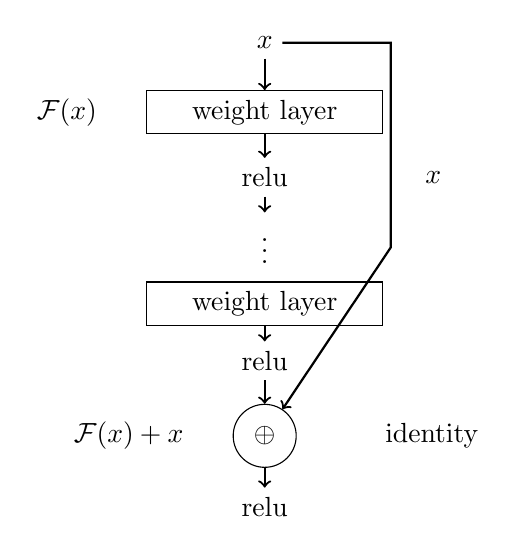
\begin{tikzpicture}[scale=0.4,
    node distance=0.4cm,
    block/.style={rectangle, draw, minimum width=3cm, minimum height=0.4cm, text centered},
    arrow/.style={->,thick},
    ]
    
    % Input x
    \node (input) at (0, 4) {$x$};
    
    % First weight layer
    \node [block, below=of input] (w1) {weight layer};
    \draw [arrow] (input) -- (w1);
    
    % First relu
    \node (relu1) [below=0.3cm of w1] {relu};
    \draw [arrow] (w1) -- (relu1);
    
    % % Second weight layer
    % \node [block, below=0.3cm of relu1] (w2) {weight layer};
    % \draw [arrow] (relu1) -- (w2);
    
    % Ellipsis (dots)
    \node (dots) [below=0.2cm of relu1] {$\vdots$};
    \draw [arrow] (relu1) -- (dots);
    
    % Third weight layer
    \node [block, below=0.1cm of dots] (w3) {weight layer};
    
    % Last relu
    \node (relu2) [below=0.2cm of w3] {relu};
    \draw [arrow] (w3) -- (relu2);
    
    % Addition node
    \node [circle, draw, minimum width=0.8cm, below=0.3cm of relu2] (add) {$\oplus$};
    \draw [arrow] (relu2) -- (add);
    
    % Identity connection (curved arrow from input to add)
    \draw [arrow] (input) -- ++(4, 0) -- ++(0, -6.5) -- (add);
    
    % Output
    \node (output) [below=0.25cm of add] {relu};
    \draw [arrow] (add) -- (output);
    
    % Labels
    \node [left=0.5cm of w1] {$\mathcal{F}(x)$};
    \node [left=0.5cm of add] {$\mathcal{F}(x) + x$};
    \node [right=1.5cm of relu1] {$x$};
    \node [right=1cm of add] {identity};

\end{tikzpicture}

\end{frame}



\begin{frame}{Skip/Residual Connection}

\small

    Prevents Vanishing or Exploding Gradients.

Consider a regular ANN:
\begin{figure}

\includegraphics[width=0.5\linewidth]{figures/multilayerblock.pdf}

If a multilayer nn can mdel $\mathcal{H}$, then it may also be able to model residual $\mathcal{H}(\xbf) - \xbf$, assuming input/ouput have same dimensions. So rather than expecting layers to model $\mathcal{H}$, we expect them to model $\Fcal(\xbf) = \mathcal{H}(\xbf) - \xbf$, and the using a skip connection, we have $\Fcal(\xbf) + \xbf$ later.
\end{figure}

So input-output mapping becomes:

\begin{align*}
\ybf = \Fcal( \xbf, \{ W_i\} ) + \xbf
\end{align*}

\footnotesize

\textbf{Reference}: He, Kaiming, Xiangyu Zhang, Shaoqing Ren, and Jian Sun. "Deep residual learning for image recognition." In Proceedings of the IEEE conference on computer vision and pattern recognition, pp. 770-778. 2016.

    
\end{frame}

\begin{frame}{Number of layers and neurons to consider}

Consider following citieria:

\begin{enumerate}


\item How does the peformance change as we increase the number of layers?
\item Do training time scale with number of layers?

\item What happens to the training performance if you add more neurons?
\end{enumerate}

\end{frame}



\begin{frame}{Early Stopping}



\begin{block}{}

Stop the training process when some conditions are fulfilled to avoid overfitting.

\end{block}

Usually adhoc, but we can establish some rules. Use validation set for early stopping.

\begin{figure}
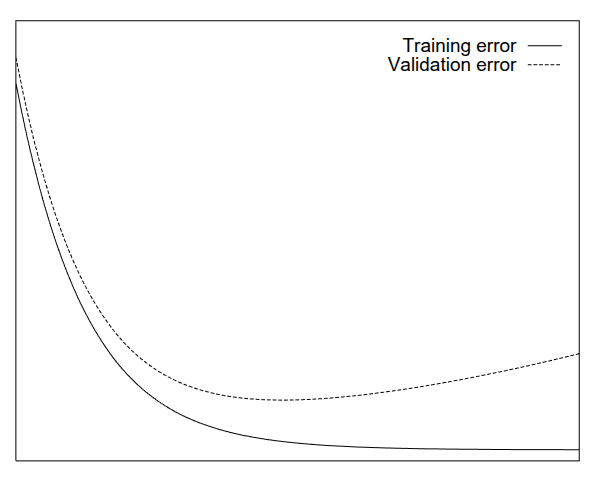
\includegraphics[width=0.5\linewidth]{figures/training_validation.png}
\end{figure}

\end{frame}



\begin{frame}{Early Stopping}




$\Lcal$ be the loss (or objective or cost) function. $\Lcal_{tr}$ be the training loss, $\Lcal_{val}$ be the validation loss. We can define the lowest validation set error obtained in epochs upto $t$ epochs:

\begin{align*}
\Lcal_{opt}(t) := \min_{t' \leq t} E_{val}(t')
\end{align*}


We can define generalization loss as 

\begin{align*}
G(t) = 100 \bigg( \frac{\Lcal_{val}(t)}{\Lcal_{opt}(t)} -1 \bigg)
\end{align*}

It  means we define generalization loss at epoch $t$ as relative increase of validation error over the minimum so far. And, we specify a stopping criteria as, \textbf{stop when generalization loss after epoch $t$ exceeds a certain threshold $\alpha$.}

\end{frame}




\begin{frame}{But let it train for a while before early stopping}



To avoid stopping while the model is still learning rapidly, we define \textbf{training progress} over a strip of length $k$:
    
    \vfill
    
    \begin{align*}
        P_k(t) &:= 1000 \cdot \left( \frac{\sum_{t'=t-k+1}^{t} E_{tr}(t')}{k \cdot \min_{t'=t-k+1}^{t} E_{tr}(t')} - 1 \right)
    \end{align*}
    
    \vfill
    
    \begin{itemize}
        \item Measures how much \textbf{average} error exceeds \textbf{minimum} error in a strip.
        \item High values indicate unstable or rapidly improving phases.
        \item Approaches zero as training stabilizes.
    \end{itemize}
\end{frame}

\begin{frame}{Stopping Criteria: Generalization vs. Progress}
    We can define a criterion using the quotient of generalization loss ($G$) and training progress ($P_k$):
    
    \vfill
    
    \begin{align*}
        PQ_{\alpha} &: \text{stop at first end-of-strip epoch } t \text{ where} \\
        &\frac{G(t)}{P_k(t)} > \alpha
    \end{align*}
    
    \vfill
    
    \begin{itemize}
        \item \textbf{Logic:} Only stop when the ratio of "error increase" to "learning speed" is too high.
        \item Assumes strips of length $k=5$ for standard measurements.
    \end{itemize}
\end{frame}


\begin{frame}{Stopping Criteria: Successive Increases}
    The \textbf{third class} of stopping criteria relies on the sign of changes in generalization error.
    
    \vfill
    
    \begin{align*}
        UP_s &: \text{stop if } UP_{s-1} \text{ stops after epoch } t - k \text{ and} \\
        &E_{va}(t) > E_{va}(t - k) \\
        UP_1 &: \text{stop after first end-of-strip epoch } t \text{ with } E_{va}(t) > E_{va}(t - k)
    \end{align*}
    
    \vfill
    
    \begin{itemize}
        \item Training stops when generalization error increases in $s$ successive strips.
        \item This assumes consecutive increases indicate the start of final overfitting.
    \end{itemize}
\end{frame}

% --- Frame 4: Advantages of UP Criteria ---
\begin{frame}{Advantages of the UP Criteria}
    \vfill
    
    \begin{itemize}
        \item \textbf{Magnitude Independent}: The decision is independent of how large the increases actually are.
        \item \textbf{Local Measurement}: Changes are measured locally rather than against global minima.
        \item \textbf{Application}: Useful in pruning algorithms where errors may remain high over long periods.
    \end{itemize}
    
    \vfill
    
    But remember, these is just one kind of early stopping example, you can design your own.
    
    \textbf{Reference:} Prechelt, Lutz. "Early stopping-but when?." In Neural Networks: Tricks of the trade, pp. 55-69. Berlin, Heidelberg: Springer Berlin Heidelberg, 2002.
\end{frame}

\begin{frame}{References and Additional Reading}

\footnotesize

\begin{enumerate}
\item He, Yulei, Guangyu Zhang, and Chiu-Hsieh Hsu. \textbf{Multiple imputation of missing data in practice: basic theory and analysis strategies}. Chapman and Hall/CRC, 2021.
\item Huang, Lei. Normalization Techniques in Deep Learning. Cham: Springer, 2022.
\end{enumerate}

\end{frame}

\begin{frame}{Learning Rate Scheduling}

\begin{block}{}

Automatically adjust the learning rate during training.

\end{block}

\begin{enumerate}
\item \textbf{StepLR:} reduces the learning rate by a fixed factor at regular intervals.
\item \textbf{ExponentialLR:} reduces the learning rate by multiplying it by a decay factor each epoch.

\item \textbf{CosineAnnealingLR:} follows a cosine curve, starting high and smoothly decreasing to a minimum value.

\item \textbf{ReduceLROnPlateau:}  monitoring validation metrics and reducing the learning rate only when improvement stops happening.
\end{enumerate}

\end{frame}

\begin{frame}{Warm-Up Scheduling}

\begin{block}{}

Warmup scheduling is a strategy used in deep learning to stabilize the training of complex neural network architectures. It addresses the trade-off between optimization stability and training speed.

\end{block}

\begin{enumerate}
\item For simplicity, the learning rate typically increases linearly during the warmup period until it reaches a specified initial maximum.

\item Once the warmup is complete, the learning rate is gradually decreased (cooled down) until the optimization process concludes.
\end{enumerate}

\end{frame}


\subsection{Optimizers}

\begin{frame}
    \subsectionpage
\end{frame}

\begin{frame}{Different Kind of Optimizers}
Gradient Descent is one of the many optimizers that can be used to optimize a function and find its minima. Some other commonly popular optimizers are
\begin{enumerate}
\item RMSProp
\item Adagrad (Adaptive Gradient)
\item SGD with Momentum
\item SGD with Nesterov Accelerated Gradient
\item AdaDelta
\item ADAM
\end{enumerate}
\end{frame}

\begin{frame}{RMSProp}
\small
\textbf{RMSProp} (Root Mean Square Propagation) is an adaptive learning rate method that divides the learning rate by an exponentially decaying average of squared gradients.

\begin{itemize}
    \item Update rule:
    \begin{multiequation}
    g_t &= \nabla_\theta J(\theta_t) \\
    v_t &= \beta v_{t-1} + (1 - \beta) g_t^2 \\
    \theta_{t+1} &= \theta_t - \frac{\eta}{\sqrt{v_t} + \epsilon} g_t
    \end{multiequation}
    \item $\eta$: Learning rate
    \item $\beta$: Decay rate (typically 0.9)
    \item $\epsilon$: Small constant for numerical stability
\end{itemize}
\end{frame}

\begin{frame}{Adagrad (Adaptive Gradient)}
\small
\textbf{Adagrad} adapts the learning rate to the parameters, performing smaller updates for frequently occurring features and larger updates for infrequent ones.

\begin{itemize}
    \item Update rule:
    \begin{multiequation}
    g_t &= \nabla_\theta J(\theta_t) \\
    G_t &= G_{t-1} + g_t^2 \\
    \theta_{t+1} &= \theta_t - \frac{\eta}{\sqrt{G_t} + \epsilon} g_t
    \end{multiequation}
    \item $\eta$: Learning rate
    \item $G_t$: Accumulated squared gradients
    \item $\epsilon$: Small constant for numerical stability
\end{itemize}
\end{frame}

\begin{frame}{SGD with Momentum}
\small
\textbf{SGD with Momentum} accelerates gradient descent by adding a fraction of the previous update to the current update.

\begin{itemize}
    \item Update rule:
    \begin{multiequation}
    g_t &= \nabla_\theta J(\theta_t) \\
    v_t &= \gamma v_{t-1} + \eta g_t \\
    \theta_{t+1} &= \theta_t - v_t
    \end{multiequation}
    \item $\eta$: Learning rate
    \item $\gamma$: Momentum term (typically 0.9)
    \item $v_t$: Velocity vector
\end{itemize}
\end{frame}

\begin{frame}{SGD with Nesterov Accelerated Gradient}
\small
\textbf{Nesterov Accelerated Gradient (NAG)} improves momentum by calculating the gradient at the estimated future position.

\begin{itemize}
    \item Update rule:
    \begin{multiequation}
    g_t &= \nabla_\theta J(\theta_t - \gamma v_{t-1}) \\
    v_t &= \gamma v_{t-1} + \eta g_t \\
    \theta_{t+1} &= \theta_t - v_t
\end{multiequation}
    \item $\eta$: Learning rate
    \item $\gamma$: Momentum term (typically 0.9)
    \item $v_t$: Velocity vector
\end{itemize}
\end{frame}

\begin{frame}{AdaDelta}
\small
\textbf{AdaDelta} is an extension of Adagrad that reduces its aggressive, monotonically decreasing learning rate.
\begin{columns}
\column{0.5\linewidth}
\begin{itemize}
    \item Update rule:
    \begin{multiequation}
    g_t &= \nabla_\theta J(\theta_t) \\
    E[g^2]_t &= \rho E[g^2]_{t-1} + (1 - \rho) g_t^2 \\
    \Delta \theta_t &= -\frac{\sqrt{E[\Delta \theta^2]_{t-1} + \epsilon}}{\sqrt{E[g^2]_t + \epsilon}} g_t \\
    E[\Delta \theta^2]_t &= \rho E[\Delta \theta^2]_{t-1} + (1 - \rho) \Delta \theta_t^2 \\
    \theta_{t+1} &= \theta_t + \Delta \theta_t
\end{multiequation}

\end{itemize}

\column{0.5\linewidth}
\begin{itemize}
    \item $\rho$: Decay rate (typically 0.9)
    \item $\epsilon$: Small constant for numerical stability
\end{itemize}
\end{columns}

\end{frame}

\begin{frame}{ADAM (Adaptive Moment Estimation)}
\small
\textbf{ADAM} combines the benefits of RMSProp and Momentum by adapting learning rates and using momentum.

\begin{columns}
\column{0.5\linewidth}
\begin{itemize}
    \item Update rule:
    \begin{multiequation}
    g_t &= \nabla_\theta J(\theta_t) \\
    m_t &= \beta_1 m_{t-1} + (1 - \beta_1) g_t \\
    v_t &= \beta_2 v_{t-1} + (1 - \beta_2) g_t^2 \\
    \hat{m}_t &= \frac{m_t}{1 - \beta_1^t} \\
    \hat{v}_t &= \frac{v_t}{1 - \beta_2^t} \\
    \theta_{t+1} &= \theta_t - \frac{\eta}{\sqrt{\hat{v}_t} + \epsilon} \hat{m}_t
\end{multiequation}
\end{itemize}

\column{0.5\linewidth}
\begin{itemize}
    \item $\eta$: Learning rate
    \item $\beta_1, \beta_2$: Exponential decay rates (typically 0.9 and 0.999)
    \item $\epsilon$: Small constant for numerical stability
\end{itemize}
\end{columns}
\end{frame}


\begin{frame}{Stabilizing Gradients: Value Clipping}
    In \textbf{value clipping}, each element of the gradient vector $g$ is independently forced into the range $[-c, c]$:
    
    \vfill
    
    \begin{align*}
        g_i \leftarrow \max(-c, \min(c, g_i))
    \end{align*}
    
    \vfill
    
    \begin{itemize}
        \item \textbf{Hard Thresholding}: Prevents any single weight update from being inappropriately large.
        \item \textbf{Effect on Direction}: Unlike norm clipping, this may change the \textit{direction} of the gradient vector.
        \item \textbf{Implementation}: Often used to prevent "jitter" in unstable phases of training.
    \end{itemize}
\end{frame}

\begin{frame}{Stabilizing Gradients: Norm Clipping}
    To prevent exploding gradients in unstable optimization problems, we rescale the gradient vector $g$ if its norm exceeds a threshold $\tau$:
    
    \vfill
    
    \begin{align*}
        g \leftarrow \text{min}\left(1, \frac{\tau}{\|g\|}\right) g
    \end{align*}
    
    \vfill
    
    \begin{itemize}
        \item \textbf{Direction Preservation}: Unlike value clipping, norm clipping maintains the direction of the update.
        \item \textbf{Synergy with Warmup}: Both techniques mitigate divergence in advanced network designs.
    \end{itemize}
\end{frame}


    \begin{frame}
        \Huge{\centerline{\color{MediumBlue}\textbf{The End}}}
    \end{frame}



\end{document}